%%%%%%%%%%%%%%%%%%%%%%% file typeinst.tex %%%%%%%%%%%%%%%%%%%%%%%%%
%
% This is the LaTeX source for the instructions to authors using
% the LaTeX document class 'llncs.cls' for contributions to
% the Lecture Notes in Computer Sciences series.
% http://www.springer.com/lncs       Springer Heidelberg 2006/05/04
%
% It may be used as a template for your own input - copy it
% to a new file with a new name and use it as the basis
% for your article.
%
% NB: the document class 'llncs' has its own and detailed documentation, see
% ftp://ftp.springer.de/data/pubftp/pub/tex/latex/llncs/latex2e/llncsdoc.pdf
%
%%%%%%%%%%%%%%%%%%%%%%%%%%%%%%%%%%%%%%%%%%%%%%%%%%%%%%%%%%%%%%%%%%%


\documentclass[runningheads,a4paper]{llncs}

\usepackage{amssymb}
\setcounter{tocdepth}{3}
\usepackage{graphicx}
\usepackage{color}
\usepackage{amsmath,amssymb,mathtools}
\usepackage{listings}
\usepackage{algorithm}
\usepackage{algorithmic}
\usepackage{centernot}
\usepackage{tikz}
\usetikzlibrary{calc}
\usetikzlibrary{shapes}
\usepackage{pgfplots}
\usepackage{pgfplotstable}


%%%%% BEGIN SPACE SAVERS %%%%%
\usepackage{times} % More compact font, allowed by lncs
\usepackage{microtype} % reduces some unnecessary spaces

% Reduces useless spacing around section headers
\makeatletter
\renewcommand\section{\@startsection{section}{1}{\z@}%
                       {-2\p@ \@plus -4\p@ \@minus -4\p@}%
                       {5\p@ \@plus 2\p@ \@minus 2\p@}%
                       {\normalfont\large\bfseries\boldmath
                        \rightskip=\z@ \@plus 8em\pretolerance=10000 }}
\renewcommand\subsection{\@startsection{subsection}{2}{\z@}%
                       {-8\p@ \@plus -4\p@ \@minus -4\p@}%
                       {4\p@ \@plus 2\p@ \@minus 2\p@}%
                       {\normalfont\normalsize\bfseries\boldmath
                        \rightskip=\z@ \@plus 8em\pretolerance=10000 }}
\renewcommand\subsubsection{\@startsection{subsubsection}{3}{\z@}%
                       {-4\p@ \@plus -4\p@ \@minus -4\p@}%
                       {-1.5em \@plus -0.22em \@minus -0.1em}%
                       {\normalfont\normalsize\bfseries\boldmath}}
\makeatother

% Reduce useless space before paragraphs
\makeatletter
\renewcommand\paragraph{\@startsection{paragraph}{4}{\z@}%
                                      {\parskip}%{3.25ex \@plus1ex \@minus.2ex}%
                                      {-1em}%
                                      {\normalfont\normalsize\itshape}}
\makeatother

% Nuclear weapon: use only if strictly needed :)
%\def\baselinestretch{0.97}

%%%%% END SPACE SAVERS %%%%%


\newcommand\x[1]{\ensuremath{\mathit{#1}}}
\newcommand\lrangle[1]{\ensuremath{\langle#1\rangle}}

\makeatletter
\providecommand{\bigsqcap}{%
  \mathop{%
    \mathpalette\@updown\bigsqcup
  }%
}
\newcommand*{\@updown}[2]{%
  \rotatebox[origin=c]{180}{$\m@th#1#2$}%
}
\makeatother


%\usepackage{url}
%\urldef{\mailsa}\path|{dwyer, mgerrard}@cse.unl.edu|    
%\newcommand{\keywords}[1]{\par\addvspace\baselineskip
%\noindent\keywordname\enspace\ignorespaces#1}

\begin{document}

\mainmatter  % start of an individual contribution

% comment macro
\newcommand{\mycomment}[1]{\textit{\textcolor{red}{#1}}}
\newcommand{\ignore}[1]{}

% first the title is needed
\title{Probabilistic Program Analysis}

% a short form should be given in case it is too long for the running head
\titlerunning{Probabilistic Program Analysis}

\author{Matthew B. Dwyer\inst{1}
\and Antonio Filieri\inst{2}\and Jaco Geldenhuys\inst{4}\and Mitchell Gerrard\inst{1}\and\\
Corina Pasareanu\inst{3}\and Willem Visser\inst{4}}
%
\authorrunning{Probabilistic Program Analysis}
% (feature abused for this document to repeat the title also on left hand pages)

% the affiliations are given next; don't give your e-mail address
% unless you accept that it will be published
\institute{University of Nebraska -- Lincoln
\and Imperial College London
\and NASA Ames Research Center
\and University of Stellenbosch
}
%Tiergartenstr. 17, 69121 Heidelberg, Germany\\
%\mailsa\\
%\url{http://www.springer.com/lncs}}

%
% NB: a more complex sample for affiliations and the mapping to the
% corresponding authors can be found in the file "llncs.dem"
% (search for the string "\mainmatter" where a contribution starts).
% "llncs.dem" accompanies the document class "llncs.cls".
%

\toctitle{Lecture Notes in Computer Science}
\tocauthor{Authors' Instructions}
\maketitle


\begin{abstract}
This paper provides a survey of recent work on adapting 
techniques for program analysis to compute probabilistic
characterizations of program behavior.  We survey how the
frameworks of data flow analysis and symbolic execution have
incorporated information about input probability distributions
to quantify the likelihood of properties of program states.
We identify cutting themes that relate and distinguish
the variety of
techniques that have been developed over the past 15 years
in this area.  In doing so, we point out opportunities for
future research that builds on the strengths of different techniques.
\keywords{data flow analysis, symbolic execution, abstract interpretation, model checking, probabilistic program, MDP}
\end{abstract}

\section{Introduction}
\label{sec:introduction}

Static program analyses calculate properties of 
the possible executions of a program without ever running the program,
and have been an active topic of study for over five decades.
Initially developed to allow compilers to generate more efficient
output programs, by the mid-1970s \cite{fosdick1976data} researchers 
understood that program analyses could be applied to fault
detection and verification of the absence of specific classes of faults.

The power of these analysis techniques, and what distinguishes them from
simply running a program and observing its behavior, is their
ability to reason about program behavior without knowing all of the
details of program execution (e.g., the specific 
input values provided to the program).
This tolerance of uncertainty allows analyses
to provide useful information when users don't know exactly how
a program will be used.

Static analyses model uncertainty 
through the use of various forms of abstraction and symbolic representation.
For example, symbolic expressions are used to encode logical constraints 
in symbolic execution~\cite{king1976symbolic}, to define abstract domains
in data flow analysis~\cite{kildall1973unified,cousot1977abstract}, and to 
capture sets of data values that constitute reachable states via
predicate abstraction~\cite{graf1997predabs}.
Nondeterministic choice is another widely used approach,
for instance, in modeling branch decisions in data flow analysis.
While undeniably effective, these approaches sacrifice potentially
important distinctions in program behavior.   

Consider a program that accepts an integer input representing
a person's income.  A static analysis might reason about the program
by allowing any integer value, or, perhaps, by applying
some simple assumption, i.e., that income must be non-negative.
Domain experts have studied income distributions and find that
incomes vary according to a generalized beta distribution 
\cite{mcdonald1984some,thurow1970analyzing}.  
With such a distribution the program can now be viewed as a 
\textit{probabilistic program} 
and, beginning with Kozen's seminal work in the early 1980s,
the semantics of such programs has long been studied 
\cite{kozen1981semantics,kozen1983probabilistic,jones1990probabilistic,morgan1996probabilistic}.

For non-probabilistic programs, it was just over six years
from Floyd's foundational work on program semantics~\cite{FLOYD67} 
to Kildall's widely-applicable static analysis framework~\cite{kildall1973unified}.
Sophisticated extensions of Kildall's work are prevalent 
today, e.g., ~\cite{lam11:_soot_java,Lattner:2004:LLVM}, and form 
the basis for modern software development environments.
For probabilistic programs, however, the development of 
static analysis frameworks has taken decades and 
they have not yet reached the level of applicability of 
their non-probabilistic counterparts.

What would such analyses have to offer?
Researchers have explored the use of probabilistic analysis
results to assess the security of software 
components~\cite{mardziel2013dynamic} and to measure side-channel 
leakage~\cite{CSF16,FSE16},
to assess program reliability~\cite{Filieri2013}, to measure program
similarity~\cite{Geldenhuys2012}, 
to characterize fault propagation~\cite{RiskAwareTransformation},
and to characterize the coverage
achieved by an analysis technique~\cite{DwyerASE11}.
\mycomment{Corina: add some more examples here about your latest work}
We believe that there are many more applications for cost-effective
and widely-applicable static analysis frameworks for probabilistic
programs.

In recent years, the term ``probabilistic program'' has been generalized 
beyond Kozen's definition in which programs draw inputs from probability 
distributions.
This more general setting permits the conditioning of program behavior by
allowning certain program runs to be rejected.  
These programs can be viewed as expressing computations over 
probability distributions rather than inputs drawn from a distribution.  
While recent work has just begun to explore the foundations of analysis for
this more general setting~\cite{claret2013bayesian,Gordon2014}, 
in this paper we consider
Kozen's original definition and analysis frameworks targetting such programs.

More specifically, we survey work on adapting data flow analysis 
and symbolic execution to use information about input distributions.
We begin with background that provides basic definitions
related to static analysis and probabilistic models.
Section~\ref{sec:overview} exposes some of the key
intuitions and concepts that cross-cut the work in this area.
The following two sections, \ref{sec:pdfa}-\ref{sec:pse}, 
survey work on probabilistic data flow analysis and probabilistic
symbolic execution.  
While we focus on analysis of imperative programs, we note that
principles exposed in our survey apply to analysis frameworks 
for functional programs as well.
Section~\ref{sec:computingprobabilities} discusses approaches that
have been developed to reason about the probability of program-related 
events, e.g., executing a path, taking a branch, or reaching a state.
We conclude with a set of open questions
and research challenges that we believe are worth pursuing.


\section{Overview}
\subsection{Scope and Background}
\label{sec:background}

This paper focuses on programs that draw input variables
from given probability distributions, or, equivalently, that make
calls on functions returning values drawn from given distributions.
The left side of Figure~\ref{fig:example} shows a method,
\texttt{m}, that we will use to illustrate concepts in this paper.     
It takes an integer variable, \texttt{x}, as input, then based on the 
results of drawing values from a Bernoulli distribution,
it either performs its computation
(which is unspecified and denoted with \texttt{...}) or triggers
an assertion. 
For the example, we might be interested in reasoning about the lack
of assertion violations.

\begin{figure}[t]
\begin{minipage}[b]{0.05\linewidth}
~
\end{minipage}%
\begin{minipage}[b]{0.25\linewidth}
\centering
\begin{lstlisting}[language=Java,numbers=left,basicstyle=\scriptsize\ttfamily]
m(int x) {
 if(drawBernoulli(0.5) == 1) {
  if(drawBernoulli(0.5) == 1) {
   if(x <= 60)
    ...
   else
    assert false
  } else {
   if(x <= 30)
    ...
   else
    assert false
  }
 } else {
  if(x <= 55)
   ...
  else
   assert false
 }
}
\end{lstlisting}
\end{minipage}%
\begin{minipage}[b]{0.3\linewidth}
\tikzstyle{every node}=[text centered, font=\scriptsize, inner sep=1pt]
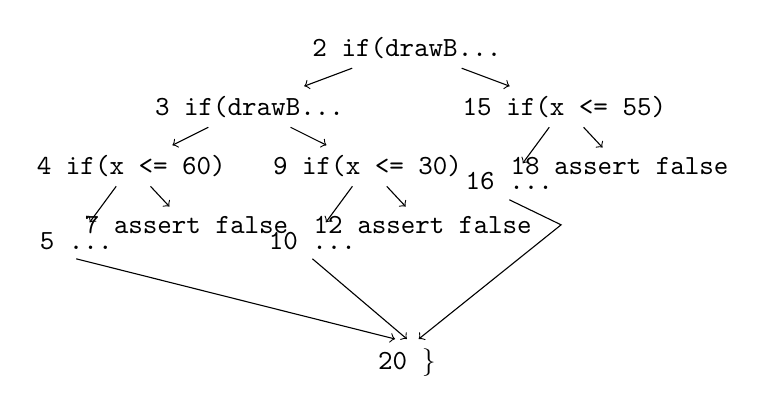
\begin{tikzpicture}[scale=0.5, level/.style={sibling distance = 40mm, level distance = 15mm}]
  \node[name=entry, xshift=0mm, yshift=20mm] {\texttt{2 if(drawB...}}
   child{
    node[xshift=-10mm] {\texttt{3 if(drawB...}}
     child{
      node[xshift=-5mm] {\texttt{4 if(x <= 60)}}
       child{
        node[name=e1,yshift=-2mm,xshift=3mm] {\texttt{5 ...}}
        edge from parent[->]
       }
       child{
        node[xshift=-3mm] {\texttt{7 assert false}}
        edge from parent[->]
       }
      edge from parent[->]
     }
     child{
      node[xshift=5mm] {\texttt{9 if(x <= 30)}}
       child{
        node[name=e2,yshift=-2mm,xshift=3mm] {\texttt{10 ...}}
        edge from parent[->]
       }
       child{
        node[name=m1,xshift=-3mm] {\texttt{12 assert false}}
        edge from parent[->]
       }
      edge from parent[->]
     }
     edge from parent[->]
   }
   child{
    node[xshift=10mm] {\texttt{15 if(x <= 55)}}
     child{
      node[name=e3,yshift=-2mm,xshift=3mm] {\texttt{16 ...}}
      edge from parent[->]
     }
     child{
      node[xshift=-3mm] {\texttt{18 assert false}}
      edge from parent[->]
     }
    edge from parent[->]
   }
;
\node[name=r,below of=entry, yshift=-30mm] {\texttt{20 \}}};
\draw[->] (e1.south) to ($(r.north)+(-3mm,0)$);
\draw[->] (e2.south) to ($(r.north)+(0,0)$);
\draw[->] (e3.south) to ($(m1.east)+(5mm,0)$) to ($(r.north)+(3mm,0)$);
\end{tikzpicture}
\end{minipage}
\caption{Example: Source Code (left) and Control Flow Graph (right)}
\label{fig:example}
\end{figure}



\subsubsection{Programs and Program Analyses}

There are many different ways to represent the execution behavior
of a program to facilitate analysis.  Immediately to the right of
the code in Figure~\ref{fig:example}, we show the control flow graph (CFG),
which explicitly represents control successor relationships between
statements.  A CFG models choice among successors as nondeterministic
choice -- depicted by the lack of labels on the edges.

We will also consider models that include probabilistic choice,
e.g., defining the probability that a branch is taken.
The left side of Figure~\ref{fig:choice} shows edge probabilities
that reflect the outcome of the Bernoulli draw on line 2. Thus the probability 
of taking the {\em then} branch is 0.5; the probability of taking 
the {\em else} branch is also 0.5.
In addition, we will consider models where the
choice of successor is defined by the semantics
of the branch condition.
The right side of Figure~\ref{fig:choice} 
shows a logical condition that 
reflects the fact that the value of parameter $x$ must be
less than or equal to $60$ for control to traverse the true branch at line 4.

\begin{figure}[t]
\begin{minipage}[b]{0.5\linewidth}
\centering
\footnotesize
\begin{lstlisting}[language=Java,basicstyle=\scriptsize\ttfamily]
m(int x) {
 if(drawBernoulli(0.5) == 1) {
  if(drawBernoulli(0.5) == 1) {
   if(x <= 60)
    ...
   else
    assert false
  } else {
   if(x <= 30)
    ...
   else
    assert false
  }
 } else {
  if(x <= 55)
   ...
  else
   assert false
 }
}
\end{lstlisting}
\vspace{-1.8in}
\hspace{1.2in}
\tikzstyle{every node}=[text centered, font=\scriptsize, inner sep=1pt]
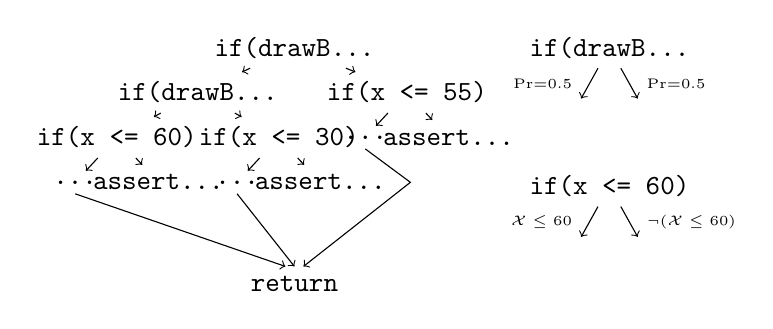
\begin{tikzpicture}[scale=0.38, level/.style={sibling distance = 12mm, level distance = 15mm}]
  \node[yshift=0mm] {\texttt{if(drawB...}}
   child{
    node[xshift=-10mm] {\texttt{if(drawB...}}
     child{
      node[xshift=-8mm] {\texttt{if(x <= 60)}}
       child{
        node[name=e1,xshift=-3mm] {\texttt{...}}
        edge from parent[->]
       }
       child{
        node[xshift=3mm] {\texttt{assert...}}
        edge from parent[->]
       }
      edge from parent[->]
     }
     child{
      node[xshift=8mm] {\texttt{if(x <= 30)}}
       child{
        node[name=e2,xshift=-3mm] {\texttt{...}}
        edge from parent[->]
       }
       child{
        node[name=m1,xshift=3mm] {\texttt{assert...}}
        edge from parent[->]
       }
      edge from parent[->]
     }
     edge from parent[->]
   }
   child{
    node[xshift=12mm] {\texttt{if(x <= 55)}}
     child{
      node[name=e3,xshift=-3mm] {\texttt{...}}
      edge from parent[->]
     }
     child{
      node[xshift=3mm] {\texttt{assert...}}
      edge from parent[->]
     }
    edge from parent[->]
   }
;
\node[name=r,yshift=-30mm] {\texttt{return}};
\draw[->] (e1.south) to ($(r.north)+(-3mm,0)$);
\draw[->] (e2.south) to ($(r.north)+(0,0)$);
\draw[->] (e3.south) to ($(m1.east)+(5mm,0)$) to ($(r.north)+(3mm,0)$);

  \node[xshift=40mm] {\texttt{if(drawB...}}
    child{
      node[yshift=-2mm, xshift=-2mm] {}
      edge from parent[->]
      node[left,xshift=-1mm] {\tiny Pr=0.5}
    }
    child{
      node[yshift=-2mm, xshift=2mm] {}
      edge from parent[->]
      node[right,xshift=1mm] {\tiny Pr=0.5}
  };

  \node[xshift=40mm,yshift=-50] {\texttt{if(x <= 60)}}
    child{
      node[yshift=-2mm, xshift=-2mm] {}
      edge from parent[->]
      node[left,xshift=-1mm] {\tiny ${\cal X} \le 60$}
    }
    child{
      node[yshift=-2mm, xshift=2mm] {}
      edge from parent[->]
      node[right,xshift=1mm] {\tiny $\neg({\cal X} \le 60)$}
  };

\end{tikzpicture}
\end{minipage}%
\vspace{0.25in}
\caption{Example}
\label{fig:example}
\end{figure}



A key concept in the program analysis frameworks we survey is
\textit{symbolic abstraction}.  A symbolic abstraction is a 
representation of a set of states.  Abstractions can be encoded
in a variety of forms, e.g., logical formulae \cite{thakur2012bilateral}, binary
decision diagrams \cite{bryant1992symbolic}, or custom representations \cite{bagnara2008parma}.  For example, the set of negative integer values 
can be defined by a predicate 
$lt0 \equiv \lambda x.x<0$ which returns true for all values in the set.
Logical combinations of such predicates can be used to define
an abstract domain, ${\cal A}$, whose elements describe sets of
possible states of the program.

While abstractions encode sets of states, \textit{abstract transformers}
compute the effect of a program statement on a set of states.  For example,
the fact that the sum of any pair of negative values is negative is
encoded as $lt0 +^\# lt0 = lt0$, where $\#$ denotes an abstract transformer
for $+$ that operates on symbolic encodings of sets.

Analyses that seek to prove the satisfaction of properties generally
define abstractions that \textit{overapproximate} the set of program
states, whereas those that seek to falsify properties generally define
abstractions that \textit{underapproximate} the set of program states.

\paragraph{Data Flow Analysis}
Data flow analysis~\cite{kildall1973unified} 
provides a framework for computing properties shared by sets of
program traces reaching a program state.  It is
common for such analyses to group together the states that share a
common control location; the computed properties attempt to characterize
the invariants over those states.

Data flow analyses are solved using a fixpoint computation which
allows properties of all program paths to be safely approximated.
Model checking~\cite{clarke1999model} is a popular verification technique
which also relies on an underlying
fixpoint computation.  Moreover, data flow
analyses operate on symbolic abstractions of program states that
can be defined by abstract interpretation~\cite{cousot1977abstract}. 
In fact, it is now well-understood that data flow analysis can be
viewed as model checking of abstract interpretations~\cite{schmidt1998data}.

An abstract interpretation is a 
non-standard interpretation of program executions over an abstract domain.  
The semantics of program statements are lifted to operate
on a set of states, encoded as an element of the abstract domain,
rather than on a single concrete state.  
Generating the set of traces for non-trivial programs is impractical;
instead, abstract states can be combined, via a meet operation, wherever
traces merge in the control flow, and loops are processed
repeatedly to compute the maximum fix point (MFP).

Data flow analysis tools and toolkits exist for popular 
languages, e.g., \cite{vallee1999soot,fink2012wala,Lattner:2004:LLVM},
and have been used primarily for program optimization and
verifying program conformance with assertional specifications.

\paragraph{Symbolic Execution}
Like data flow analysis, symbolic execution~\cite{king1976symbolic,clarke1976system} 
performs a non-standard interpretation of program executions using 
a symbolic abstraction of program states.
Symbolic execution records symbolic expressions encoding the
values of program memory for each program location.  
A \textit{path condition}
accumulates symbolic expressions that encode branch constraints 
taken along an execution.

Sequences of program statements are interpreted by applying the operation
at each program location to update the values of program
variables with expressions defined over symbolic variables.
An operation that reads from an input generates a fresh symbolic
variable which represents the set of possible input values.
When a branching statement is encountered, the symbolic expression, $c$, 
encoding the branch condition is computed and a check is performed
to determine whether the current trace---encoded by the path condition---can be
extended with $c$ or $c$'s negation.  
This is done by formulating the constraints
as a satisfiability query; if the formula encoding branch constraints
is satisfiable, then there must exist an input that will follow the trace.
The trace is extended following the feasible branch outcomes, usually
in a depth-first manner.

In the example of Figure~\ref{fig:example}, on the leftmost path through
the control flow graph, when symbolic execution reaches the 
final branch it will record the condition ${\cal X} \le 60$, where
${\cal X}$ models the unknown value of input $x$.  This condition describes the
set of input values that will trigger execution of this path---as long
as both Bernoulli trials yield a value of 1.

In practice symbolic execution computes an underapproximation of 
program behavior.
Programs with looping behavior that is determined by input values 
may result in an infinite symbolic execution.
For this reason, symbolic execution is
typically run with a (user-specified) bound on the search depth, thus
some paths may be unexplored.   Moreover, there may be path constraints
for which efficient satisfiable checking is not possible.  Variants of
symbolic execution~\cite{godefroid2005dart,sen2005cute,song2008bitblaze},
called concolic execution, address this problem by replacing problematic 
constraints with equality constraints between variables 
and values collected while executing the program along the trace.

Symbolic execution tools and toolkits exist for many popular 
languages~\cite{pasareanu2010symbolic,godefroid2005dart,jamrozik2013generating,cadar2008klee}
and have been used primarily for test generation and fault detection.

\subsubsection{Probabilities and Probabilistic Models}

There is an enormous literature on probabilistic reasoning and statistics
that can be brought to bear in program analysis.  
In this paper, we consider two types of discrete time probabilistic models:
Markov chains and Markov decision processes (MDP)~\cite{Puterman:MDP94}.

Both models rely on the concept of a probability distribution.
A \textit{probability distribution} a probability distribution is a function 
that provides the probability of occurrence of different possible outcomes 
in an experiment.
%over a set is given by a function
%that maps each of the set's subsets to some real number between 0 and 1;
%this number represents the probability of a given subset being the outcome
%of a random experiment.
The sum of the probabilities for all outcomes is 1.

\ignore{
A \textit{distribution} over a set $S$ is given by a 
function $\pi : S \rightarrow [0,1]$ where
$\sum_{s \in S} \pi(s) = 1$.  For $s \in S$,
$\pi(s)$ is said to be the probability of $s$ -- it is
sometimes written Pr(s).
The set of distributions for $S$ is denoted $D_S$.

A Markov chain is a labeled transition system,
$(S,I,L,R)$, where $S$ is a set of states,
$I \subseteq S$ is a set of initial states (if there is a single
such state we denote it $s_0$), 
$L : S \rightarrow 2^{AP}$ is a function that assigns
sets of atomic propositions to a state, and
$R : S \rightarrow D_S$ defines for a given state
the probability of moving to another state.
The probability of executing a sequence of states $s = s_0, ..., s_n$, 
is $Pr(s) = \prod_{i \in [0,n-1]} R(i)(i+1)$.

Given a distinguished set of goal states, $G \subseteq S$,
we can define $Tr(G) = \{s_0, \ldots, s_n \vert s_0 \in I \wedge
s_n \in G \wedge \forall i \in [0,n-1] : R(s_i)(s_{i+1}) > 0$
as the traces reaching a $G$-state.
The probability of reaching a state in 
a set of goal states, $G$, is $Pr(G) = \sum_{s \in Tr(G)} Pr(s)$.
}

A Markov chain is a labeled transition system that, given some
state, defines the probability of moving to another state, according 
to a probability distribution.
The probability of executing a sequence of states is then the
product of the transition probabilities between the states.
The model fragment in the upper right corner of 
Figure~\ref{fig:example} depicts a Markov chain fragment.
It defines, for the set of states 
that are at the first line in the program, 
a 0.5 probability of transitioning to 
the state representing the beginning of the then block,
and similarly for the beginning of the else block.  The
distribution indicates a 0 probability of moving to any
other state.

For this small example, if we were to assume a probability
distribution on the input $x$, then it would be possible
to compute the probability of taking every edge in the CFG.   
This would be a Markov chain model of {\tt m} and it would replace
all nondeterministic choices in the CFG with probabilistic choices.

There are many situations where the removal of nondeterministic
choices is impractical or undesirable.  For example, if the input
distribution of $x$ is unknown, then retaining nondeterministic
choices for the conditionals which test that value would yield a
faithful program model.  In addition, it may be desirable, for
efficiency of analysis, to abstract program behavior, and that
abstraction may make it impossible to accurately compute the 
probability of a transition.  

Including nondeterminism in a probabilistic state
transition model yields a Markov decision process (MDP).
An MDP adds an additional structure, $A$, that defines
a set of (internal) actions which are used to model the
selection among a set of possible next-state probability distributions.
When traversing a path in an MDP, in each state, a choice
from $A$ must be made in order to determine how to transition,
probabilistically, to a next state.   That sequence of choices
\ignore{$\sigma \in A^*$,} is termed a \textit{policy} for the MDP.
Given a policy, an MDP reduces to a Markov chain.
One of the advantages of using MDP an lies in its ability to provide upper and
lower bounds on the behavior of the modeled system (discussed
in the following section).
\ignore{
For an MDP, let $Pr^{\sigma}(G)$ be the probability of reaching
a $G$-state from an initial state using schedule $\sigma$;
this is equivalent to $Pr(G)$ for the Markov chain induced
by fixing the schedule.  We can then define 
$Pr^+(G) = \max_{\sigma} Pr^{\sigma}(G)$
and
$Pr^-(G) = \min_{\sigma} Pr^{\sigma}(G)$
as the maximum and minimum probabilities of reaching a $G$-state
in the MDP over the set of all possible schedules.  
}

\section{Overview}
\label{sec:overview}

The literature on incorporating probabilistic techniques into 
program analysis is large and growing, technically deep, and quite
varied.  In this paper we cannot hope to cover all of it, but our
intention is to expose key similarities and differences between 
families of approaches and, in doing so, provide the reader with
intuitions that are often missing in the detailed presentation of
techniques, quite helpful in understanding them.

\subsection{Where do the probabilities come from?}
There are two perspectives adopted in the literature.
Programs are implicitly probabilistic because the distributions
from which input values are drawn are not specified in the program,
but are characteristic of the execution environment.
Alternately, programs are explicitly probabilistic in that the statements
within the program define the input probability distributions.
More generally a program might combine both implicit and explicit
probabilistic calls.  Method $m$ in Figure~\ref{fig:example}
is an example of such a combined probabilistic program.

It is possible to transform explicit probabilistic constructs,
by introducing auxiliary input variables and then specifying
their distributions.   For the example, this would result
in the addition of two integer input variables 
\begin{quote}
\texttt{m(int x, int b1, int b2) \{...} 
\end{quote}
where the two instances of
\texttt{drawBernoulli(0.5)} expressions would be replaced
by \texttt{b1} and \texttt{b2}, respectively.  The input
distribution for these auxiliary inputs would then be specified
as a set of pairs,
\[
\{ (\lambda x.x<0,0), (\lambda x.x=0,0.5), (\lambda x.x=1,0.5), (\lambda x.x>1,0) \}
\]
where the first component defines the characteristic function
of a set of values and the second component defines the probability
of a value in that set.

\subsection{What does the analysis compute?}
There are two perspectives adopted in the literature.
One can view a probabilistic program as a transformer on probability
distributions and compute the probability distribution, over the
concrete domain, that holds at a program state.
Alternatively, one can view a probabilistic program as a program 
whose inputs happen
to vary in some principled way and compute program properties, 
properties of sets of concrete domain elements, along with a characterization
of how that property varies with varying input.
Within these approaches there are types of approximations
computed for probabilities.  It is common to compute upper bounds
on probabilities for program properties, but lower bounds can 
be computed as well.  In addition, it is possible to estimate the
probability within some margin of error -- an approach that several
techniques explore -- and it is even possible to compute the probability
\textit{exactly} if certain restrictions hold on the program and distributions.

\ignore{
example showing a negation function with drawBernoulli(0.25)
and how it transforms a distribution

show a program that tests whether the absolute value of a number
is greater than 5 where the input is distributed according to N(0,1)
}


\subsection{Handling abstraction expressed through non-determinism}
Any analysis that hopes to scale will invariably be forced to overapproximate
behavior.  As explained earlier in static analyses it is common
to model such overapproximation using non-deterministic choice.
Across all of the analysis techniques we have surveyed, MDPs
have been in these situations since they naturally mix probabilistic
and non-deterministic choice.   
An important consequence of using MDPs is that it is no longer possible
to compute a single probabilistic characterization of a property.
Instead analyses can compute, across the set of all possible sequences
of non-deterministic choice outcomes, the minimal and maximal 
probabilities for a property to hold.

If the minimal probability for a property of interest lies above 
a desired probability threshold, then regardless of how the non-determinism
is resolved the property is guaranteed to hold with the desired 
threshold.  If that is not the case, but the maximal probability for
a property of interest lies above a desired threshold, then there
there is a schedule to resolve the non-determinism that satisfies
the property with at least the desired property.


\section{Probabilistic Approaches to Program Analysis}
\section{Probabilistic Data Flow Analysis}
\label{sec:pdfa}

As we will see in all sections, probabilistic data flow
analysis moves from the true/false nature of its classical
counterpart to the probably-true/probably-false nature of
a static analysis extended with probabilities.
The shift from the qualitative to the quantitative allows
you to incorporate probabilistic information into the
analysis in different ways.

\subsection{Control Probabilities}

Initial work in extending data flow analysis 
techniques with probabilities did not consider
the semantics of the program; instead, already-given probabilities 
were attached to nodes in that program's control flow graph.  
The goal was to predict the probability of an expression evaluating 
to some value or type at runtime, which could 
allow you to perform useful program optimizations.

This approach begins with a control flow graph where each edge $e$ is 
mapped to the probability that $e$ is taken during execution.
The sum of all probabilities leaving any control flow node must be 1
(excepting the exit node).
These probabilities may be obtained through heuristics, profiling,
or some static analysis.
Imagine an execution trace following some path along the edges of
the control flow graph.
The probability of executing that trace is expressed as the product of 
edge probabilities along this path.
So the probability of executing some program point can be seen as the
summation of the probabilities of traces which can reach that program
point.

\mycomment{Mitch: insert figure to make explanation more concise}

Within this bag of execution traces which reach point $u$, we want to 
find the portion of traces which satisfy some data flow fact $d$.  
The ratio of the satisfying portion to the size of the trace bag
gives us the probability of fact $d$ holding at point $u$.

To compute this expected frequency, Ramalingam uses a slightly
modified version of Kildall's dataflow analysis framework
~\cite{ramalingam1996data}.
Instead of the usual semilattice with an idempotent meet
operation, we use the non-idempotent addition operator.
The restricted properties of the meet operation can be
relaxed because instead of computing invariant dataflow
fact, we only want the summation of probabilities of all
traces reaching a certain point.
The expected frequencies may now be computed as the least
fixed point using the same iterative algorithm presented
in the background; the quantity becomes a
{\sl sum-over-all-paths} instead of a {\sl meet-over-all-paths}.

\mycomment{Mitch: Ramalingam also deals with a slight variation
on a lattice, but his variation is close enough to a traditional
lattice that I don't think we need to mention this?}

Ramalingam's work assumes execution history does not matter 
(the analysis is path insensitive).
Later work adds some path sensitivity \cite{mehofer2001novel}, 
but as both frameworks deals with exploded control flow graphs, a fully 
path-sensitive approach is not tractable.

\subsection{Data Probabilities}

Within the last 15 years, research in probabilistic data flow analysis
began incorporating probabilistic information directly into
the semantics of a program \cite{monniaux2000abstract}.
This is typically done using a variation on Kozen's 
probabilistic semantics \cite{kozen1981semantics} 
alongside traditional data flow techniques.
Embedding probabilities into the semantics allows probabilistic
information to influence how both control {\sl and} data structure
probabilities are computed during the analysis.

The remaining approaches in this section permit probabilistic
information to be defined as either an environment property
(i.e., distribution given for an input) or in the type of
an expression (i.e., rand call).
We examine techniques that use the framework of abstract
interpretation.

How do the classical abstract domains work in a
probabilistic setting?
We will focus on one technique developed by Monniaux
that requires little change to the classical domain 
\cite{monniaux2001backwards}.
The key difference between the classical and the probabilistic 
case is that in the probabilistic case, 
an abstract domain has a weight attached to any of its subsets.
More formally
$\mathcal{A}_p \equiv \mathcal{P}(\mathcal{A} \times \mathcal{R}^+)$, 
i.e., a set of pairs $(a,w)$ where $a \in \mathcal{A}$ implicitly
defines a set of concrete values, $\gamma(a)$, such that
$\forall c \in \gamma(a) : Pr(c) \le w$.

The valuation of any element in the concrete domain then 
becomes the additive composition of weights of points in 
the concrete domain which are represented by elements in
the abstract domain.
For instance if $ap \in \mathcal{A}_p$ is such that
$(a_i,w_i) \in ap$ and 
$(a_j,w_j) \in ap$ then $c \in \gamma(a_i) \wedge
c \in \gamma(a_j) \implies Pr(c) \le w_i + w_j$.
The concretization function maps from a set of abstract
values to a weight function.

We cannot go over the details of probabilistic semantics here, but there
are a few modifications to the abstract semantics of a
traditional imperitive program (see Hankin's WHILE language) 
which we will point out.
One is the addition of a random number generator primitive; it
is possible and straightforward to approximate a safe upper
bound on this generator.
Approximations on loop semantics are dealt with in a safe way
using ``suitable" widening operators instead of fixed points.

Conditionals can be seen as filtering
the abstract domain between those execution environments which
satisfy the conditional and those which falsify the conditional. 
The difference in the probabilistic abstract environment with weights 
is that the filter is only applied to the first component of
the tuple (the traditional elements of an abstract domain), 
and leaves the weight unchanged.
For instance, consider the abstract domain of an interval of 
integers defined by the tuple, $([-5,5],0.1)$. 
If this domain holds before a conditional of 
{\tt if(x<0)\{...\}}, after applying the filter on the true branch, 
we get $([-5,-1],0.1)$. 
After applying the filter on the false branch, we get $([0,5],0.1)$.
The space is reduced; the weights remain the same.

An example will be helpful (simplified from Monniaux's (2004)).
We will work with the abstract domain of intervals in $\mathcal{R}$,
Consider the following C-like program, where {\tt centered\_uniform()}
and {\tt abs(x)} return a {\tt double} uniformly distributed in 
$[-1,1]$ and the absolute value of {\tt x}, respectively.

{\tt double x;\\
     .../* A */\\
     x = centered\_uniform();\\
     if(abs(x) <= 1) \{ /* B */ \}}

We want to find a weight function which, for any element in the
concrete domain, sums up the weights of the corresponding elements
in the abstract domain.

\mycomment{Mitch : should our example include overlapping intervals
to highlight the ``summation" aspect of the weight function?}

This correctness criterion is given as an upper bound on the
probability of some outcome in the program, e.g. {\sl the
probability of violation $\phi$ is less than $0.0001\%$}.
Dually, other approaches have
used lower probability bounds as their correctness criterion.

\subsection{Handling nondeterminism}
\mycomment{Matt: I am working in this section - reading on last paper before
I edit}

There are variations of uncertainty,
and not every program property should be modeled by a
probability distribution.
For instance, a user may exploit an unlikely control sequence
in a vending machine to get free candy bars. 
If word gets out, the probability of
this exploited behavior occurring is poorly modeled by a uniform 
random distribution.
It is better to treat this kind of input nondeterminisitically.

In Monniaux's semantics, choices that can be tied to a known
distribution are cleanly separated from those that cannot.
A nondeterministic choice allows for independent outcomes, and
this is modeled by lifting the singleton outcomes of deterministic
semantics to powersets of outcomes.
In the probabilistic setting, the elements of this powerset are
tuples of the abstract domain and the associated weight, defined
above.
So for any nondeterminstic choice, the resulting computation 
is safely modeled by one of these tuples.

\subsection{More and varied probabilistic data flow analyses}

Bounds on the probability of a state property have been well studied.
Di Pierro et al. \cite{di2013probabilistic} aim to estimate the probability of a property,
rather than bound it.  They formulate their an abstract 
domain over vector spaces, instead of lattices, and use
the Moore-Penrose pseudo-inverse instead of the usual fixed point.
While shown to be effective on small programs, the space
complexity of vector space encodings and lack of tool support
have not yet demonstrated the scalability of the approach.
More recent work has explored computing an alternative probabilistic
property called {\sl expectation invariants} \cite{chakarov2014expectation}.
This approach uses an iterative data flow analysis to 
compute a bound on the long-run expected value of
some program expression, e.g. $E[f(uniform(0,10))] < 7$ states that,
over a sufficiently large number of runs, when $f$ is called with
a uniformly distributed number in the range $[0,10]$, it will return
an average value less than 7.

The idea of a ``probabilistic program" has been generalized from
Kozen's original semantics to include conditioning on program
observations~\cite{Gordon2014}.
In this setting, the program implicitly specifies a probability 
distribution conditioned on these stated observations.
Data flow analyses have recently been adapted to perform Bayesian
inference on this new class of probabilistic 
programs~\cite{claret2013bayesian}.  

\section{Probabilistic Symbolic Execution}
\label{sec:pse}

\subsection{Introduction}
\begin{itemize}
\item symex produces PCs and interested in SAT/UNSAT and solutions
\item now we are interested in number of solutions, given a profile
\item ISSUE: we assume uniform, but where will non-uniform be described?
\item we can use model counting to count solutions for a PC (given uniform)
\item dividing the solution count by the domain count gives probability of the PC holding
\item call this probabilistic symbolic execution
\end{itemize}

\subsection{Applications}

\begin{itemize}
\item knowing the probability of a PC
\item low-level: probability of a path, reaching a location, returning a value, failing an assertion,... 
\item that can lead to...
\item reliability of a piece of code
\item program understanding
\item program equivalence
\item domain coverage
\end{itemize}

\subsection{Approach}

{\bf following is just placeholder sentences}

Note that the symex algorithm from section blah (background) produces path conditions along the way, which we can then use to do model counting, ...

However, in order to allow us to sample a space of behaviours, i.e. paths, when all paths cannot be exhaustively analysed, we rather use the algorithm below, which samples fully executed symbolic paths. 

\begin{minipage}{0.5\textwidth}
\begin{algorithm}[H]
\renewcommand{\thealgorithm}{}
\floatname{algorithm}{Alg.}
\caption{{\tt pse}$(l,m,\phi)$}
\label{symexe}
\begin{algorithmic}
 \REPEAT
  \STATE $p \gets {\tt symsample}(l_0, m_0, \x{true})$
  \STATE $\x{processPath}(p)$
 \UNTIL {$\x{stoppingSearch}(p)$}
\end{algorithmic}
\end{algorithm}
\end{minipage}
\begin{minipage}{0.5\textwidth}
\begin{algorithm}[H]
\renewcommand{\thealgorithm}{}
\floatname{algorithm}{Alg.}
\caption{{\tt symsample}$(l,m,\phi)$}
\label{symexe}
\begin{algorithmic}
 \IF{$\x{stoppingPath}((\phi)$} 
 \RETURN $\phi$
 \ENDIF
 \WHILE{$\neg branch(l)$}
   \STATE $m \gets m\lrangle{v, e}$
   \STATE $l \gets next(l)$
 \ENDWHILE
 
 \STATE $c \gets (m[\x{cond}(l)]$
 
 \IF{$\x{selectBranch}(c,\phi)$}
   \RETURN {\tt symsample}$(\x{target}(l), m, \phi \wedge c)$
 \ELSE
   \RETURN {\tt symsample}$(\x{next}(l), m, \phi \wedge \neg c)$
 \ENDIF
\end{algorithmic}
\end{algorithm}
\end{minipage}

\subsubsection{stoppingpath}

First explain stoppingPath, since it is arguably also part of symex itself: finite paths not an issue, but infinite paths, i.e. loops on input, must be stopped  {\bf but this needs to move to background really, since the algorithm there is never going to terminate}

\subsubsection{selectBranch}

\begin{itemize}
\item If we sample exhaustively then we could pick branches any which way we want to, but we have to record which ones we have picked to allow termination [ note we will explain this in the processPath section this requires us to explain the counting and subtracting values etc.
\item to do a proper monte carlo simulation we need to consider the counts of each branch
\item could be elaborate here and use heuristics
\item what if the branch is nondeterministic?
\end{itemize}

\subsubsection{stoppingSearch}

\begin{itemize}
\item now we have to consider the domain coverage, i.e. stopping when we have searched a pre-defined level of the domain, this needs to include the discussion about gray paths
\item also need to talk about the statistical approach from FSE paper, hopefully Antonio can do this, the SA contingent is not capable!
\item need to mention sample with replacement here as well
\end{itemize}

\subsubsection{processPath}
\begin{itemize}
\item it checks the property of interest
\item Now we need to discuss the parts about storing the branch and the counts etc. i.e. the non replacement and termination issues
\end{itemize}

\subsection{Nondeterminism}

Here we will not say much but refer to our previous work in the ICSE paper and then the more elaborate approach in the ASE paper.

\subsection{Open Issues}

Can't think of a good name for this section now.

\begin{itemize}
\item Domains for counting: reals, non-linear, structures, strings, \#sat
\item distributed algorithms
\item discussion about input partitions if not going in the next section by Corina
\end{itemize}


\subsection{Computing Program Probabilities}
\label{sec:computingprobabilities}

Computing probabilities for probabilistic program analysis can usually be reduced to computing the probability of satisfying a boolean constraint over the program variables. In this section we will introduce some of the basic techniques currently used in program analysis. 

To simplify the notation, we will focus on implicit probabilistic constructs, assuming the program under analysis has input variables $V=\{v_1, v_2, \dots, v_n\}$, where $v_i$ has domain $d_i$ and comes with a probability distribution $\mathcal{P}_i: d_i \to [0, 1]$. The input domain $D$ is defined as the cartesian product of the domains $d_i$, while the input distribution $\mathcal{P}$ is defined as the joint distribution over all the input variables $\prod_i \mathcal{P}_i(\bar{v_i})$. Given a constraint $\phi: V \to \{true, false\}$, our goal is to compute the probability $Pr(\phi)$ of satisfying $\phi$ given the input domains and probability distributions. This problem is usually referred to as model counting, when the input domains are countable, or solution space quantification, when the input domains are modeled as uncountable (e.g., abstracting floating-point numbers as reals).

\subsubsection{Exact and numeric computation}\label{sec:computingprobabilitiesExact}

% OUTLINE
%	\begin{enumerate}
%		\item Finite domains
%			\begin{enumerate}
%				\item Linear integers (Latte, Barvinok, Omega for negation; used in our works)
%				\item Strings (bounds: \url{http://www.comp.nus.edu.sg/~shweta24/publications/smc\_pldi14.pdf} ; automata-based exact and upperbounds: \url{http://www.cs.ucsb.edu/~bultan/publications/model-counting.pdf}; we should also check the related work thereof)
%				\item Data structures (icse13 and spin15)
%				\item Sat and smt (\url{http://arxiv.org/pdf/1306.5726v3.pdf}, \url{http://arxiv.org/pdf/1411.0659.pdf}; these papers should have been published, we should check related work in there)
%			\end{enumerate}
%		
%		\item Uncountable domains
%			\begin{enumerate}
%				\item Symbolic and numerical integration (interesting, but symbolic does not scale apart from a few simple cases, while numeric suffers for large cardinality of input domains; however: general, available off-the-shelf, parallelizable for numerical)
%			\end{enumerate}
%	\end{enumerate}

\paragraph{Finite domains.} 

If the input domain is finite, the classical formulation of probability can be used to reduce the computation of $Pr(\phi)$ to a counting problem (here we assume a uniform distribution over all the possible input values, i.e., each valid input has the same probability):
%
\begin{equation}\label{eq:counting}
	Pr(\phi) = \frac{\sharp(\phi \land D)}{\sharp(D)}
\end{equation}
%
\noindent where $\sharp(\cdot)$ counts the number of inputs satisfying the argument constraint; $D$ has been overloaded to represent the finite domain as a constraint ($\sharp(D)$ is a short form for the size of the domain)\footnote{More precisely, Equation~\eqref{eq:counting} represents the probability of satisfying the constraint $\phi$ conditioned on the fact that the input is within the prescribed domain $D$.}. For example, considering a single integer input variable $x$ taking values between $1$ and $10$ uniformly, $\sharp(D)=10$ and $\sharp(x\leq5 \land D)=5$, leading to a $0.5$ probability of satisfying the constraint.

Efficient implementations of $\sharp(\cdot)$ are available for several classes of model counting problems:

\begin{itemize}
	\item \textbf{Linear integer arithmetic}: the conjunction of linear constraints over a finite integer domain geometrically defines a multi-dimensional lattice bounded by a convex polytope~\cite{de2008computationalGeometry}. To count the number of points composing this structure, an efficient solution has been proposed by Barvinok in~\cite{barvinok1994polynomial}. This algorithm is grounded on the construction of generating functions suitable for solving the counting problem in polynomial time, with respect to the number of variables and the number of constraints. Notably, besides the number of bits required to represent the numerical values, the complexity of this algorithm does not depend on the actual size of the variable domains. This makes the computation feasible for very large input domains, allowing its application to probabilistic program analysis. Several implementations of this algorithm are available, the two most popular being LattE~\cite{LattESoftware} and Barvinok~\cite{verdoolaegesoftware}. When disjunctions appear in the constraint, these have to be preprocessed before applying Barvinok's algorithm (e.g., using the Omega library~\cite{Omega1996}). This normalization increases the overall complexity of model counting, however, several optimizations can be leveraged to reduce the computational effort.
%(we will discuss some later in Section~\ref{sec:computingprobabilitiesOptimizations}) 
Barvinok's algorithm has been used for probabilistic program analysis in \cite{Geldenhuys2012,Filieri2013,Filieri2015}.

	\item \textbf{Bounded data structures}: data structures are usually composed of a structural dimension (e.g., lists or trees) and a payload stored in each node of the structure. The level of decoupling between structure and payload differs case by case---for example, a list of integers may be sorted or not. Early work on complexity analysis explored the use of generating functions for representing the number of valid instances of a given data structure without explicitly enumerating them (e.g.,~\cite{flajolet1985mathematical}). However, despite its computational efficiency, this approach requires a significant amount of human work, because the construction of these generating functions can hardly be automatically inferred from the source code. For the sake of generality, early work in probabilistic program analysis~\cite{Filieri2013} used an enumeration-based approach, such as Korat~\cite{Korat2002}. This technique relies on the formalization both of the invariants characterizing the valid structures and of the constraints to be counted as executable boolean methods, and then generates all the instances for which these methods return true. The generation is enhanced with smart pruning techniques to reduce the actual exploration space, although their complexity still leaves most realistic programs out of reach. A recent approach proposed in~\cite{Filieri2015} decouples the structural part from the payload, employing the partial enumeration of the former and the use of more efficient model counting techniques for the latter, whenever possible. For example, in an acyclic sorted list of integers between 1 and 10, having at most 3 elements would require the enumeration of 4 different structural configurations (including the empty list) and the evaluation of 8 linear integer constraints (which can be computed with Barvinok's algorithm), instead of exploring all 1111 possible instances.

	\item \textbf{Regular expressions}: a variety of practically relevant constraints on strings can be formalized as matching with a regular expression~\cite{Luu2014,Aydin2015}. If the (maximum) length of the string is bounded, the number of instances matching a regular expression can be counted exactly with an automata-based approach. The regular expression is first transformed into the corresponding accepting automata. Then, an exponential generating function is automatically constructed to count the accepting runs of the automata up to a certain length, without the need to enumerate all of them explicitly. The technique is actually more general and can be used for any constraint whose satisfaction can be reduced to counting the accepting runs of a finite state automata. For more general constraints, called pseudo-relational, the exact count is not computable, though its value can be bounded in a finite interval, allowing, in some cases, for best- or worst-case analysis~\cite{Aydin2015}.
	
\ignore{
	\item \textbf{SAT and SMT}: \mycomment{TBD (\url{http://arxiv.org/pdf/1306.5726v3.pdf}, \url{http://arxiv.org/pdf/1411.0659.pdf}; these papers should have been published, we should check related work in there)}
}

\end{itemize}


\paragraph{Floating-point numbers.} 
Floating-point numbers are usually abstracted as real numbers for analysis purposes. Computing the probability of satisfying a constraint over reals requires refining Equation~\ref{eq:counting} to cope with the density of the domain. In particular, the counting function $\sharp(\phi)$ has to be replaced by the integration of an indicator function on $\phi$, i.e., a function returning $1$ for all the inputs satisfying $\phi$ \cite{Borges2014}. This integration can be performed exactly only for a limited number of cases---those where symbolic integration is possible. For all the other cases, only numerical integration is possible. A number of commercial and open-source tools can be used for this purpose, however, 1) numerical computations are accurate only up to a certain bound, and 2) they do not scale when the cardinality of the input domain grows. In the latter case, sampling-based methods are preferable. 

\paragraph{Handling input distributions.} 
For finite domains, we assume, without loss of generality, the input distribution to be specified on a finite partition $D^1, D^2, \dots, D^n$ of the input domain $D$ (i.e., $\cup_i D^i \equiv D$ and $D^i \cap D^j \neq \emptyset \implies i=j$) via the probability function $Pr(D^i)$. We assume elements within the same set $D^i$ to have the same probability. The case of uniform distribution described so far corresponds to the partition with cardinality 1, i.e., the whole domain.
 
Since the elements of the partition are disjoint by construction, we can exploit the law of total probability to extend Equation~\eqref{eq:counting} to include the information about the input distribution:
%
\begin{equation}\label{eq:countingInputDistribution}
	Pr(\phi) = \sum_i \frac{\sharp(\phi \land D^i)}{\sharp(D^i)} \cdot Pr(D^i)
\end{equation}
%
\noindent where $D^i$ has again been overloaded to represent the constraint of an element belonging to $D^i$.

Formalizing the input distribution on a finite partition of the input domain is general enough to capture every valid distribution on the inputs, including possible correlations or functional dependencies among the input variables. However, the finer the specification of the input distribution, the more complex the computation of Equation~\eqref{eq:countingInputDistribution}, which, in the worst case, may require the computation of $|D|$ summands \cite{Borges2014}. While this worst case is unlikely to occur (partially due to the optimization strategies described later), more efficient probability computations are possible which employ distribution-aware sampling-based methods, described in the next section.

\subsubsection{Sampling-based methods}\label{sec:computingprobabilitiesSampling}
Exact methods can suffer from two main limitations: 1) generality with respect to input domains and constraint classes and 2) scalability, either due to the intrinsic complexity of the algorithm used or to the discretization of the input distributions. In many cases, sampling-based methods may be used to leverage both limitations.

In this section we will present sampling-based methods for quantifying the probability of satisfying arbitrarily complex floating-point constraints. We will briefly discuss how to generalize to different domains at the end of the section.

Sampling-based probability computations rely on the application of Monte Carlo methods for estimating the probability of satisfying a given constraint. Monte Carlo estimation is a well-developed field in Statistics, with countless applications in science and engineering~\cite{robert2013monte}. In this section, we will review the basics of some Monte Carlo estimation techniques used in probabilistic program analysis. % while in Section~\ref{sec:computingprobabilitiesOptimizations} we will show how this general techniques can be tailored to probabilistic program analysis for more efficient quantification procedures.

\paragraph{Hit-or-miss Monte Carlo.}

As in the previous section, we will first introduce this quantification technique assuming a uniform input distributions over a convex domain. Consider for example the constraint $v_1 \leq -v_2 \land v_2 \leq v_1$, where both $v_1, v_2 \in [-1, 1] \cap \mathbb{R}$. For each value of $v_1$ and $v_2$, the constraint can either be true or false. To estimate the probability of satisfying the constraint (and in turn of violating it), we can define a suitable probabilistic model and then run a set of experiments to estimate its parameters.

A suitable probabilistic model to represent the binary true/false outcome of an experiment is a Bernoulli distribution~\cite{pestman1998mathematical}. This is a parametric distribution with a single parameter, call it $p$, representing the probability of observing the true outcome; the complementary outcome, false, will have probability $1-p$.

The simplest way to estimate $p$ consists in generating $n$ independent random values for $v_1$ and $v_2$ and count how many of those values satisfy the constraint. More precisely, we can define an estimator $\hat{P}$ for the parameter $p$ which is the ratio between the number of experiments returning true and the total number of experiments, $n$. The most important properties of this estimator (that can be justified, for example, by the central limit theorem~\cite{pestman1998mathematical}) are its expected value $E[\hat{P}]$, which is the most likely estimate, and its variance $Var[\hat{P}]$, which is an index of the uncertainty we have about our estimate after the experiments. Formally:
%
\begin{equation}\label{eq:mleEstimator}
	E[\hat{P}] = \bar{x} \qquad Var[\hat{P}] = \frac{\bar{x} \cdot (1-\bar{x})}{n}
\end{equation}
%
\noindent where $\bar{x}=\sum_{i=1}^n x_i$ and $x_i$ is $1$ if the $i$-th experiment returned true and $0$ otherwise.

The estimator $\hat{P}$ has two important properties: it is unbiased, i.e., its expected value converges to the actual probability of satisfying the constraints when the number of experiments grows; it is consistent, i.e., its variance (and in turn, our uncertainty about the result) decreases to 0, in this case linearly (as can be noted by the denominator $n$ in Equation~\eqref{eq:mleEstimator}). 

From the perspective of probabilistic program analysis, these two properties can be used to guarantee the asymptotic correctness of the computed probability, as well as to quantify the convergence of the estimation process. The variance can indeed be used to provide probabilistic guarantees on the correctness of the result in the form of confidence intervals~\cite{pestman1998mathematical} (assuming $n$ is large enough):
%
\begin{equation}\label{eqConfidenceInterval}
	Pr\Big( \bar{x} - z_{\frac{\alpha}{2}} \cdot \sqrt{\frac{\bar{x} \cdot (1-\bar{x})}{n}} \ \leq p \leq \ \bar{x} + z_{\frac{\alpha}{2}} \cdot \sqrt{\frac{\bar{x} \cdot (1-\bar{x})}{n}} \Big) = 1-\frac{\alpha}{2}
\end{equation}
%
\noindent where $z_{\frac{\alpha}{2}}$ is the $1-\frac{\alpha}{2}$ quantile of the standard Normal distribution~\cite{pestman1998mathematical}. For example, if we want to have a confidence of $99.9\%$ on our estimation, we will pick $z_{\frac{\alpha}{2}}=3.08$ and keep collecting samples until the length of the interval is acceptably small, i.e., the accuracy of the result is acceptable.

Hit-or-miss Monte Carlo is the simplest estimation method suitable for our problems. However, its convergence rate is usually worse than more sophisticated techniques such as crude Monte Carlo or Markov chain Monte Carlo~\cite{Robert2005MCBook}. It is also possible to reduce the variance of the estimator with convenient sampling procedures (in place of uniform random sampling), such as stratified or importance sampling~\cite{Robert2005MCBook}. More sophisticated techniques exists when the actual value of $p$ to be estimated is close to the extremes (0 or 1), in particular, slice sampling (or splitting) has been successfully used in probabilistic model checking~\cite{importanceSamplingSMC,splittingSMC,statisticalModelChecking}. Finally, while Equation~\eqref{eqConfidenceInterval} can be used as a stopping criteria for sampling, it is grounded on fairly conservative assumptions; tighter bounds can be used to determine a priori the number of samples needed to guarantee some required accuracy and confidence level, the most popular being Chernoff-Hoeffding's bound~\cite{hoeffding1963probability,approximatePMC,statisticalModelChecking}. When checking if the computed probability of satisfying a constraint is sufficiently accurate, estimation methods can be replaced by statistical hypothesis testing, which is usually more efficient~\cite{pestman1998mathematical}. Finally, the estimator we presented in this section is a maximum likelihood estimator, defined according to frequentist probability theory; Bayesian estimation can be used as well, providing a different perspective on the problem---one that allows for the inclusion of prior knowledge on the expected result (when available) of estimation or hypothesis testing~\cite{Robert2007BayesianChoice,gelman2003bayesian}.



\paragraph{Distribution-aware sampling.} So far we have assumed that inputs are distributed uniformly within their domain. When different distributions are specified for the input variables, the hit-or-miss Monte Carlo algorithm presented above can still be applied, though the samples from input variables should be taken according to their specified input distributions.

Efficient sampling algorithms exist for the most common continuous and discrete distributions, with off-the-shelf implementations for several programming languages (e.g.,~\cite{commonsMath3} for Java). While a survey of ad-hoc methods for random number generation is beyond the scope of this paper (the interested reader can refer, e.g., to~\cite{gentle2013random}), we will briefly recall a general sampling method that can be used to reduce sampling from arbitrary distributions to sampling from a uniform one. 

Assume our goal is to take a sample from a distribution $D$, e.g., a Gaussian distribution describing the inputs received by a temperature sensor. This distribution has a cumulative distribution function $CDF_D(x)$ representing the probability of observing a value less than or equal to $x$~\cite{pestman1998mathematical}. The value of the CDF is trivially bounded between 0 and 1, for $x\to -\infty$ and $x \to \infty$, respectively. Furthermore, assuming every possible outcome has a strictly positive probability, as is the case for most distributions used in practice, the CDF is strictly monotonic and invertible; let us denote its inverse $CDF_D^{-1}(\cdot)$. A general method to reduce sampling from $D$ to sampling from a Uniform distribution is called \emph{inverse CDF sampling} or \emph{inverse transform sampling} and is composed of the following three steps:

\begin{enumerate}
	\item generate a random sample $u$ from the Uniform distribution on $[0,1]$
	\item find the value $x$ such that $CDF_D(x)=u$, i.e., $CDF_D^{-1}(u)$
	\item return $x$ as the sample from $D$
\end{enumerate}

For most practically used distributions, the inverse CDF can be computed efficiently, allowing more general input distributions to be used in sampling-based probability computation methods. Slight variations of inverse CDF sampling allow you to additionally sample from truncated distributions~\cite{cohen1991truncated}, i.e., when a probability distribution is restricted to a specific domain (e.g., the input temperature has a Gaussian distribution with a certain mean and variance, but is restricted to the range $[0,100]$), which is common in probabilistic program analysis. 

In some cases, the input variables are not probabilistically independent. For example, the temperature and the altitude measured by input sensors of an airplane might be correlated with one another, since higher altitudes usually correspond to lower temperatures. Whenever variables are not independent, their values have to be sampled as tuples from a multidimensional probability distribution. While the sampling approach discussed so far is also conceptually applicable to multidimensional distributions, it is usually computationally more expensive to compute the CDF and its inverse in higher dimensions. More sophisticated sampling techniques are preferred in this case, such as Gibbs sampling~\cite{Robert2005MCBook}.

As a final remark, while discretization can be used to obtain arbitrarily accurate approximations of complex distributions (over both integer and real numbers), the complexity of the probability computation method described in Section~\ref{sec:computingprobabilitiesExact} is exponential in the resolution of discretization, e.g., if a program has 5 input variables and the domain of each of them is split into 3 intervals, the size of the domain partition is $5^3$. When the number of variables grows, obtaining fine grained discretization of their probability distributions may become computationally too expensive. Distribution-aware sampling can be leveraged to avoid both this exponential explosion and the need to define a priori a discretization resolution~\cite{2015-fse-qcoral}.


\paragraph{Beyond floating-point numbers.}
The framework of sampling-based probability computation described in this section is theoretically applicable to domains other than purely numeric ones. However, its practical implementation requires the ability to generate random inputs from these domains, possibly according to the input distributions specified by the developers. Random test case generation has developed effective techniques to generate random inputs for realistic programs. However, most of the techniques developed in this area do not provide any guarantee on the distribution of the generated inputs, possibly biasing the estimation process. 

Sampling-based methods have been proposed for model counting of SAT problems (e.g., in~\cite{satCounting01,biere2009handbook,journalscorrMeel14}, also with distribution-aware approaches~\cite{chakraborty2014distribution}) and SMT problems (e.g., in~\cite{countingSMT}), while stochastic grammars can be used to generate random strings according to specified distributions~\cite{stochasticGrammars}.



%	\begin{itemize}
%		\item Sampling from uniform distributions (base case, best we can if no input distribution is available; based on classic probability, i.e., count success over total)
%		\item Discretization of non-uniform distributions (useful when a finite number of usage scenarios are available; can approximate any distribution with arbitrary accuracy; most straightforward when inferring distributions from past executions, i.e., histograms; it does not scale for fine-grained approximations)
%		\item Distribution-aware sampling (quite straightforward for distributions over numerical domains; requires more complex, unbiased, input generation techniques when sampling from other domains, e.g., data structures, but similar to random testing; scalability issues when sampling correlated input variables)
%      
%		\item Monte Carlo methods
%			\begin{itemize}
%				\item Hit or miss Monte Carlo
%				%\item \mycomment{Anto: Mention Crude montecarlo for integration? Gibbs and MCMC sampling will be just mentioned; especially MCMC is used by the MSR guys}
%				\item Frequentist and Bayesian estimators (used in prob. model check.)
%					\begin{itemize}
%						\item historically frequentist first, with static bounds (based on Chernoff's) for prob MC; then sequential ratio tests, still frequentist.
%						\item Bayesian from CMU
%					\end{itemize}
%				\item The variance issue and convergence acceleration techniques (just a paragraph with some refs):
%					\begin{itemize}
%						\item Importance sampling (used in prob. model check.)
%						\item Importance slicing (used in prob. model check.)
%					\end{itemize}
%
%				\item Exploiting he law of total probability for composing different estimators: Interval constraints propagation (PLDI14) and statistical/exact (FSE14)
%				\item Dealing with nondeterminism (freq and bayesian in prob MC, ASE14)	
%			\end{itemize}
%			
%			\item approximate $\sharp$-sat and $\sharp$-smt (\url{http://arxiv.org/pdf/1306.5726v3.pdf}, )
%	\end{itemize}


\ignore{
\subsection{Optimizations for PPA}\label{sec:computingprobabilitiesOptimizations}

While model counting and solution space quantification are general problems, their application to probabilistic program analysis can often be improved exploiting the additional information specific to this application field.

We briefly report in this section two techniques able to 1) exploit variables dependency to reduce the complexity of model counting and solution space quantification and 2) combine interval constraint propagation and stratified sampling to increase the accuracy of sampling-based probability computation, and in turn its convergence rate.

\paragraph{Divide and conquer.}
The complexity of all the model counting and solution space quantification techniques proposed in this section depends on the number of variables involved in the constraints to be quantified. Let us assume such constraints are provided in disjunctive normal form and that there is no intersection between the solution spaces of any pair of disjuncts (this is form is quite natural for most constraints analyzed in PPA, usually requiring low computational overhead for normalization). Since there is no intersection between the disjuncts, the solution space for each of them can be quantified separately and than summed up to obtain the result for the whole disjunction.

Let us focus on a single disjunct $\phi \equiv \phi_1 \land \phi_2 \land \dots \land \phi_n$ predicating on the variables $\{v_1, v_2, \dots, v_m\}$, i.e., for each $v_i$ there exists at least one conjunct $\phi_j$ predicating on its value. Our goal is to divide the quantification of the solution space of $\phi$ in a set of independent problems involving only a subset of the variables appearing in $\phi$. 

The central idea is that constraints in $\phi$ identify a dependency relation ($\textit{dep}$) among the constrained variables that can be formalized as follows (let $v_i$, $v_j$, and $v_k$ be variables in $\phi$ and $\phi_i$ be a conjunct in $\phi$):
\begin{itemize}
	\item $\forall v_i \ \textit{dep}(v_i,v_i)$
	\item $\forall v_i,v_j$ if there exist a conjunct $\phi_i$ predicating on both $v_i$ and $v_j$, then $\textit{dep}(v_i,v_j)$
	\item $\forall v_i,v_j,v_k$ $\textit{dep}(v_i,v_j) \land \textit{dep}(v_j,v_k) \implies \textit{dep}(v_i,v_k)$
\end{itemize}

The intuitive meaning of the $\textit{dep}$ relation is that if $\textit{dep}(v_i,v_j)$ then the values assumed by $v_i$ in a program run affect the values that can be assumed by $v_j$ towards the satisfaction of $\phi$. For example, from $\{x>5 \land y=x+5\}$ we deduce that the value of $y$ is affected by the values of $x$, and vice versa. The relation $\textit{dep}$ is an equivalence relation, thus it induces a partition on the set of variables appearing in $\phi$. For this reason, we can rewrite $\phi$ as the conjunction of the subsets $\phi_{[v]}$, each of whom collects all the constraints involving a variable in the equivalence class of $\textit{dep}$ represented by $v$. Such conjuncts are logically separated, hence it can be proved that $\textit{Pr}(\phi)= \prod_{v} \textit{Pr}(\phi_{[v]})$. 

For example, let $\phi$ be $\{x>2 \land y<5\}$, its probability can be computed as $\textit{Pr}(\phi)=\textit{Pr}(x>2) \cdot \textit{Pr}(y<5)$. The computation of the two probabilities on the right-hand side of this equality can be performed independently and each of them involves only one variable, reducing the effort of counting in a multidimensional space or taking samples from multidimensional distributions. Furthermore, the result of each subproblem can be cached and reused, with significant benefits in practical applications~\cite{Filieri2013}.


\paragraph{Interval constraint propagation and stratified sampling.}
Despite their generality, sampling-based methods for computing probability may suffer slow convergence rate. Several techniques have been established in statistics to mitigate this general issue~\cite{Robert2005MCBook}. Besides these techniques, the specificity of the problems we face in PPA can be exploited to define even more effective variance reduction technique.

Recall the example we introduced in Section~\ref{sec:computingprobabilitiesSampling}: we aim at quantifying the probability of satisfying the constraint 
$v_1 \leq -v_2 \land v_2 \leq v_1$, where both $v_1, v_2 \in [-1, 1] \cap \mathbb{R}$. Figure~\ref{fig:stratifiedICP} shows the domain and the solution space for this problem, with $v_1$ on the x-axis and $v_2$ on the y-axis. Using hit-or-miss Monte Carlo to solve this problem requires throwing random samples for $v_1$ and $v_2$ within their domain (i.e., from within the square), and computing the ratio between those falling within the shadowed triangle (i.e., satisfying the constraints) and the total number of samples. Geometrically, this corresponds to estimating the ratio between the area of the triangle and the area of the square (which is 1/4).

\begin{figure}[h!]\label{fig:stratifiedICP}
  \centering
      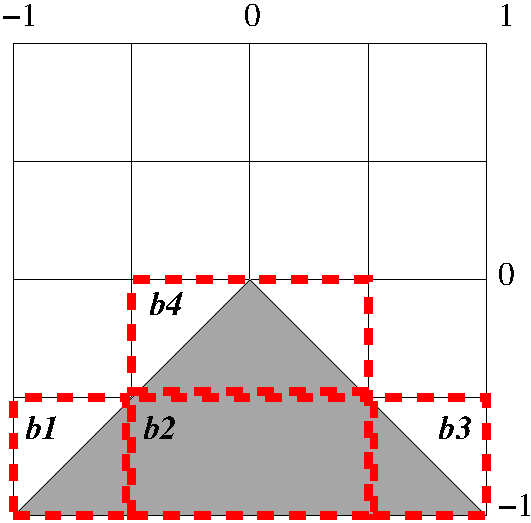
\includegraphics[width=3cm]{triangle}
  \caption{Example of ICP-based domain partitioning.}
\end{figure}

Looking at the figure it is evident that some regions of the domain do not contain solutions, i.e., the probability of satisfying the constraint within those regions is identically 0, without any estimation uncertainty. Intuitively, since we have an exact information about a fraction of the domain, we can confine the estimation, and consequently the uncertainty of estimation, only on the remaining part of the domain. This intuition can be systematized combining two techniques: interval constraint propagation and stratified sampling. 

Interval constraint propagation (ICP) is a algorithmic technique to compute interval solutions to equality and inequality numerical constraints. The input of ICP is a set of $n$ variables, each one defined on a convex domain, and a conjunction of numerical constraints; its output is a set of $n$-dimensional non-overlapping boxes whose union contains all the values of the variables satisfying all the constraints. Each box is essentially an hyperplane bounding a portion of the domain that contains solutions for the problem plus, possibly, other points that do not satisfy the constraint. Looking again at Figure~\ref{fig:stratifiedICP}, the application of ICP to our constraint produces the four 2-dimensional red boxes, whose union contains all the solutions. ICP can thus be used to partition the input domain into a set of regions, where each region may 1) contain no solutions, 2) contain only solutions, or 3) contain both solutions and values that do not satisfy the constraint. In the first two cases computing the probability will trivially lead to 0 and 1, respectively, without any uncertainty (i.e., zero variance). In the third case, sampling is needed to estimate the fraction of solution points.

When we have local results for each region in the domain partition, the second step is to compose these local information to obtain the probability estimate for the whole domain. Stratified sampling is a statistical techniques allowing to compose the local estimators of each region of the domain into a global estimator for the initial problem~\cite{Robert2005MCBook}. This computation is essentially a weighted sum of the local estimators, where the weight is the size of the region divided by the size of the domain. If we call $\hat{P}_i$ the local estimator of the $i$-th region and $w_i$ the ratio between the size of the $i$-th region and the size of the domain, exploiting the properties of expected value and variance for a sum of independent random variables~\cite{pestman1998mathematical}, we obtain for the global estimator $\hat{P}$ the following properties:

\begin{equation}\label{eq:stratifiedSampling}
	E[\hat{P}]=\sum_i w_i \cdot E[\hat{P}_i] \qquad Var[\hat{P}] = \sum_i w_i^2 \cdot Var[\hat{P}_i]
\end{equation}

The variance for the regions containing no solutions is trivially 0, thus the variance of the global estimator is reduced by the squared weight of these regions. Furthermore, for regions containing only solutions, the sampling-based probability computation will return variance 0 as well (recall Equation~\eqref{eq:mleEstimator}). Thus, fixed the total number of samples, the uncertainty on the global estimator with stratified sampling is always smaller or equal than the one we can obtain by applying Monte Carlo estimation on the whole domain, without partitions (this is a general result for stratified sampling~\cite{Robert2005MCBook}). 

The effectiveness of this approach depends on how much of the domain can be pruned out by the adopted ICP technique. This approach has been implemented in~\cite{Borges2014}, using the open-source ICP solver RealPaver~\cite{granvilliers2006tomas} for floating-point constraints, showing a significant reduction of the estimator variance on several realist programs, and, in turn, a faster convergence rate of the sampling-based probability computation. A combination of this technique with the previous divide and conquer strategy has been further developed in~\cite{2015-fse-qcoral} for a finer focusing of the sampling effort on the constraints and regions mostly affecting the variance of the global estimator, obtaining even faster convergence rates.






}







%\section{Specifying and Inferring Probability Distributions}
\label{sec:probspecs}

\section{Open Questions and Future Directions}
\label{sec:future}

Some possible things to discuss:
\begin{enumerate}
\item tools: tools support for prob. data flow analysis is really lacking
\item building a robust and flexible counting tool: that mixes methods, that cancompute prob. estimates with bounds, etc.
\item hybrid approaches: could we identify portions of a state
space that could be analyzed exactly through symex and then fold
that information back into mc/dfa approaches to boost their precision
\item inference: while we don't cover it in this paper, a key feature of
the most recent prob. programming languages is conditioning in the form
of an "observe" statement.  This functions exactly like an "assume" 
statement and could be used to drive backtracking in mc/symex.  Work
would have to be done to renormalize the prob. measures as in existing
approaches.
\item ... add more here ...
\end{enumerate}


\bibliographystyle{splncs03}
\bibliography{ppa}

\end{document}
